\documentclass[12pt,
	a4paper,
	bibliography=totocnumbered,
	listof=totocnumbered, 
	headinclude,
	captions=tableheading, 
	numbers=noenddot]{scrbook}

% Backend needs to match the used one, you can choose between {biber,bibtex}
\usepackage[backend=bibtex, sorting=none, style=alphabetic]{biblatex}
\usepackage[english, ngerman]{babel}
\usepackage[utf8]{inputenc}

\usepackage{minted}
\usepackage{tikz}
\usepackage{float}
\usepackage{url}
\usepackage[hidelinks]{hyperref}
\usepackage{ifthen}
\usepackage{caption}
\usepackage{listings}
\usepackage{graphicx}
\usepackage{svg}
\usepackage{currfile}
\usepackage{acronym}
\usepackage{fancyvrb}
\usepackage{geometry}
\usepackage{tabularx}
\usepackage{float}
\usepackage{amsmath}
\usepackage{amsfonts}
\usepackage{amssymb}
\usepackage[headsepline, automark]{scrlayer-scrpage}
\usepackage{booktabs}
\usepackage{multirow}
\usepackage{threeparttable}
\usepackage{makecell}
\usepackage{csquotes}
\usepackage{seqsplit}
\usepackage{lipsum}


% --------------------
% PACKAGE SETTINGS
% --------------------

% Library
\addbibresource{bib/literature.bib}
% Tikz
\usetikzlibrary{matrix,chains,positioning,decorations.pathreplacing,arrows}
% Graphics
\graphicspath{{./pictures/}}

% Colours
\definecolor{javared}{rgb}{0.6,0,0} % for strings
\definecolor{javagreen}{rgb}{0.25,0.5,0.35} % comments
\definecolor{javapurple}{rgb}{0.5,0,0.35} % keywords
\definecolor{javadocblue}{rgb}{0.25,0.35,0.75} % javadoc
\definecolor{gray}{rgb}{0.6,0.6,0.6}

% Intented verbatim env
\DefineVerbatimEnvironment{indentVerbatim}{Verbatim}{frame=leftline, framesep=-.75cm, numbers=left, breaklines=true}
\DefineVerbatimEnvironment{indentVerbatimX2}{Verbatim}{frame=leftline, framesep=-1.6cm, numbers=left, breaklines=true}
\DefineVerbatimEnvironment{indentVerbatimOnly}{Verbatim}{frame=leftline, numbers=left, breaklines=true, samepage=true}

% --------------------
% STYLE SETTINGS
% --------------------

\clearpairofpagestyles
\automark[chapter]{chapter}
% Comment in if you want Section names in Heading instead of Chapter
% \automark*{section}
\ihead{\headmark}
\ohead{\pagemark}
\renewcommand*\chapterpagestyle{scrheadings}


% \usepackage[T1]{fontenc}
% \usepackage{microtype}
% \usepackage{libertine}%  serif and sans erif
% \usepackage[libertine]{newtxmath}
% \usepackage[scaled=0.85]{beramono}%% mono
% \usepackage{relsize}
% \usepackage{calc}
% \usepackage{changepage}
% \usepackage{enumitem}
% \usepackage{fvextra}
% \usepackage[autostyle]{csquotes}
% \usepackage[onehalfspacing]{setspace}
% \usepackage{siunitx}
% \usepackage{subcaption}
% \usepackage[dvipsnames]{xcolor}
% \usepackage{cleveref}
% \usepackage{pgfplots}
% \usepackage{pgfplotstable}
% \usepackage{csquotes}
% \usepackage{xargs}
% \usepackage{setspace}
% \usepackage[printonlyused]{acronym}
% \usepackage{subfig}
% \usepackage{floatflt}
% \usepackage[usenames,dvipsnames]{color}
% \usepackage{colortbl}
% \usepackage{paralist}
% \usepackage{array}
% \usepackage{parskip}
% \usepackage[right]{eurosym}
% \usepackage[subfigure,titles]{tocloft}
% \usepackage{wrapfig}
% Subfile with File and Ratio as parameter
\newcommand\subfilelogo[3]{%
\def\LOGOFILE{#2}%
\def\RATIO{#3}%
\subfile{#1}%
}

\renewcommand\frontmatter[2]{
    \subfilelogo{./title/title-page}{#1}{#2} % Titelblätter 
    \thispagestyle{empty}
    \cleardoublepage
    \thispagestyle{empty}
    \cleardoublepage
    \pagenumbering{Roman}
    \subfile{./title/abstract} % Abstract
    \thispagestyle{empty}
    \tableofcontents % Inhaltsverzeichnis
    \clearpage
}

\def\backmatter{
  \chapter{Abkürzungsverzeichnis} % Wenn english: Abbreviations
  \subfile{./chapters/acronyms}
    \listoffigures
    \listoftables
    \printbibliography
    \subfile{./title/explanation} % Erklärung (Arbeit selbstständig verfasst)
}

% Listing for Pagebreaks usage
\newenvironment{longlisting}{\captionsetup{type=listing}}{}

% Uncomment this option if you dont want empty pages between chapters
% \KOMAoptions{twoside=false}


\begin{document}

\selectlanguage{ngerman}

\newcommand{\Dname}{Vorname Nachname} % Hier den Namen des Bearbeiters eintragen
\newcommand{\Dnummer}{Matrikelnummer} % Hier die Matrikelnummer eintragen
\newcommand{\Dtitel}{Titel der Arbeit} % Hier den Titel eintragen. Ggf. muss dieser getrennt werden
\newcommand{\Darbeit}{Bachelorarbeit,Masterarbeit} % Hier die Art der Abschlussarbeit eintragen
\newcommand{\Dprofa}{Prof. Dr. Wolfgang Hommel} % Hier den Aufgabensteller eintragen
\newcommand{\Dprofb}{Prof. Dr. Zweiter Prüfer} % Hier den Zweitprüfer eintragen
\newcommand{\Dbetreuera}{Betreuer 1} % Hier den Betreuer 1 eintragen
\newcommand{\Dbetreuerb}{Betreuer 2} % Hier den Betreuer 2 eintragen (meist alphabetisch). Falls nicht vorhanden, leer lassen. Ggf. auf der Titelseite löschen.
\newcommand{\Dbetreuerc}{Externer Betreuer} % Hier den Betreuer 3  bzw. externen Betreuer eintragen. Falls nicht vorhanden, leer lassen. Ggf. auf der Titelseite löschen.
\newcommand{\Dday}{01.01.2022} % Hier das Abgabedatum eintragen
\newcommand{\Dversion}{Draft vom \today} % Wenn kein Draft mehr, sondern Endversion, dann ``Draft vom \today'' löschen

% --------------------------------------------------------------------------------------
% Cover page and Some general Pages required for thesis
% --------------------------------------------------------------------------------------
\frontmatter


% --------------------------------------------------------------------------------------
% Main Content
% --------------------------------------------------------------------------------------
\mainmatter

%!TEX root = ../main.tex
\chapter{First}
\label{chap:first}

This is chapter 1

\lipsum[1-5]
\documentclass[../main]{subfiles}
\begin{document}

\chapter{Second}
\label{chap:second}

This is chapter 2

\lipsum[1-5]

\end{document}
%!TEX root = ../main.tex
\chapter{Third}
\label{chap:third}

This is chapter 3
%!TEX root = ../main.tex
\chapter{Fourth}
\label{chap:fourth}
This is chapter 4

\documentclass[../main]{subfiles}
\begin{document}

\chapter{Fifth}
\label{chap:fifth}

This is chapter 5

\end{document}
\documentclass[../main]{subfiles}
\begin{document}

\chapter{Sixth}
\label{chap:sixth}

This is chapter 6

\end{document}

% Comment this out before release
\documentclass[../main]{subfiles}
\begin{document}

\chapter{Examples}
\label{chap:examples}

\section{First Example}
\label{chap:first_example}
This is a citation \cite{buch}, this a double citation \cite{buch, buch}.

\subsection{Sub Example}
\label{chap:second_example}

You can reference other chapters or sections by \ref{chap:first_example} 
You can also reference an acronym by \ac{cmyk}


\vspace{5mm}
\begin{figure}[htbp]
	\centering
	\begin{minipage}{0.7\linewidth}
	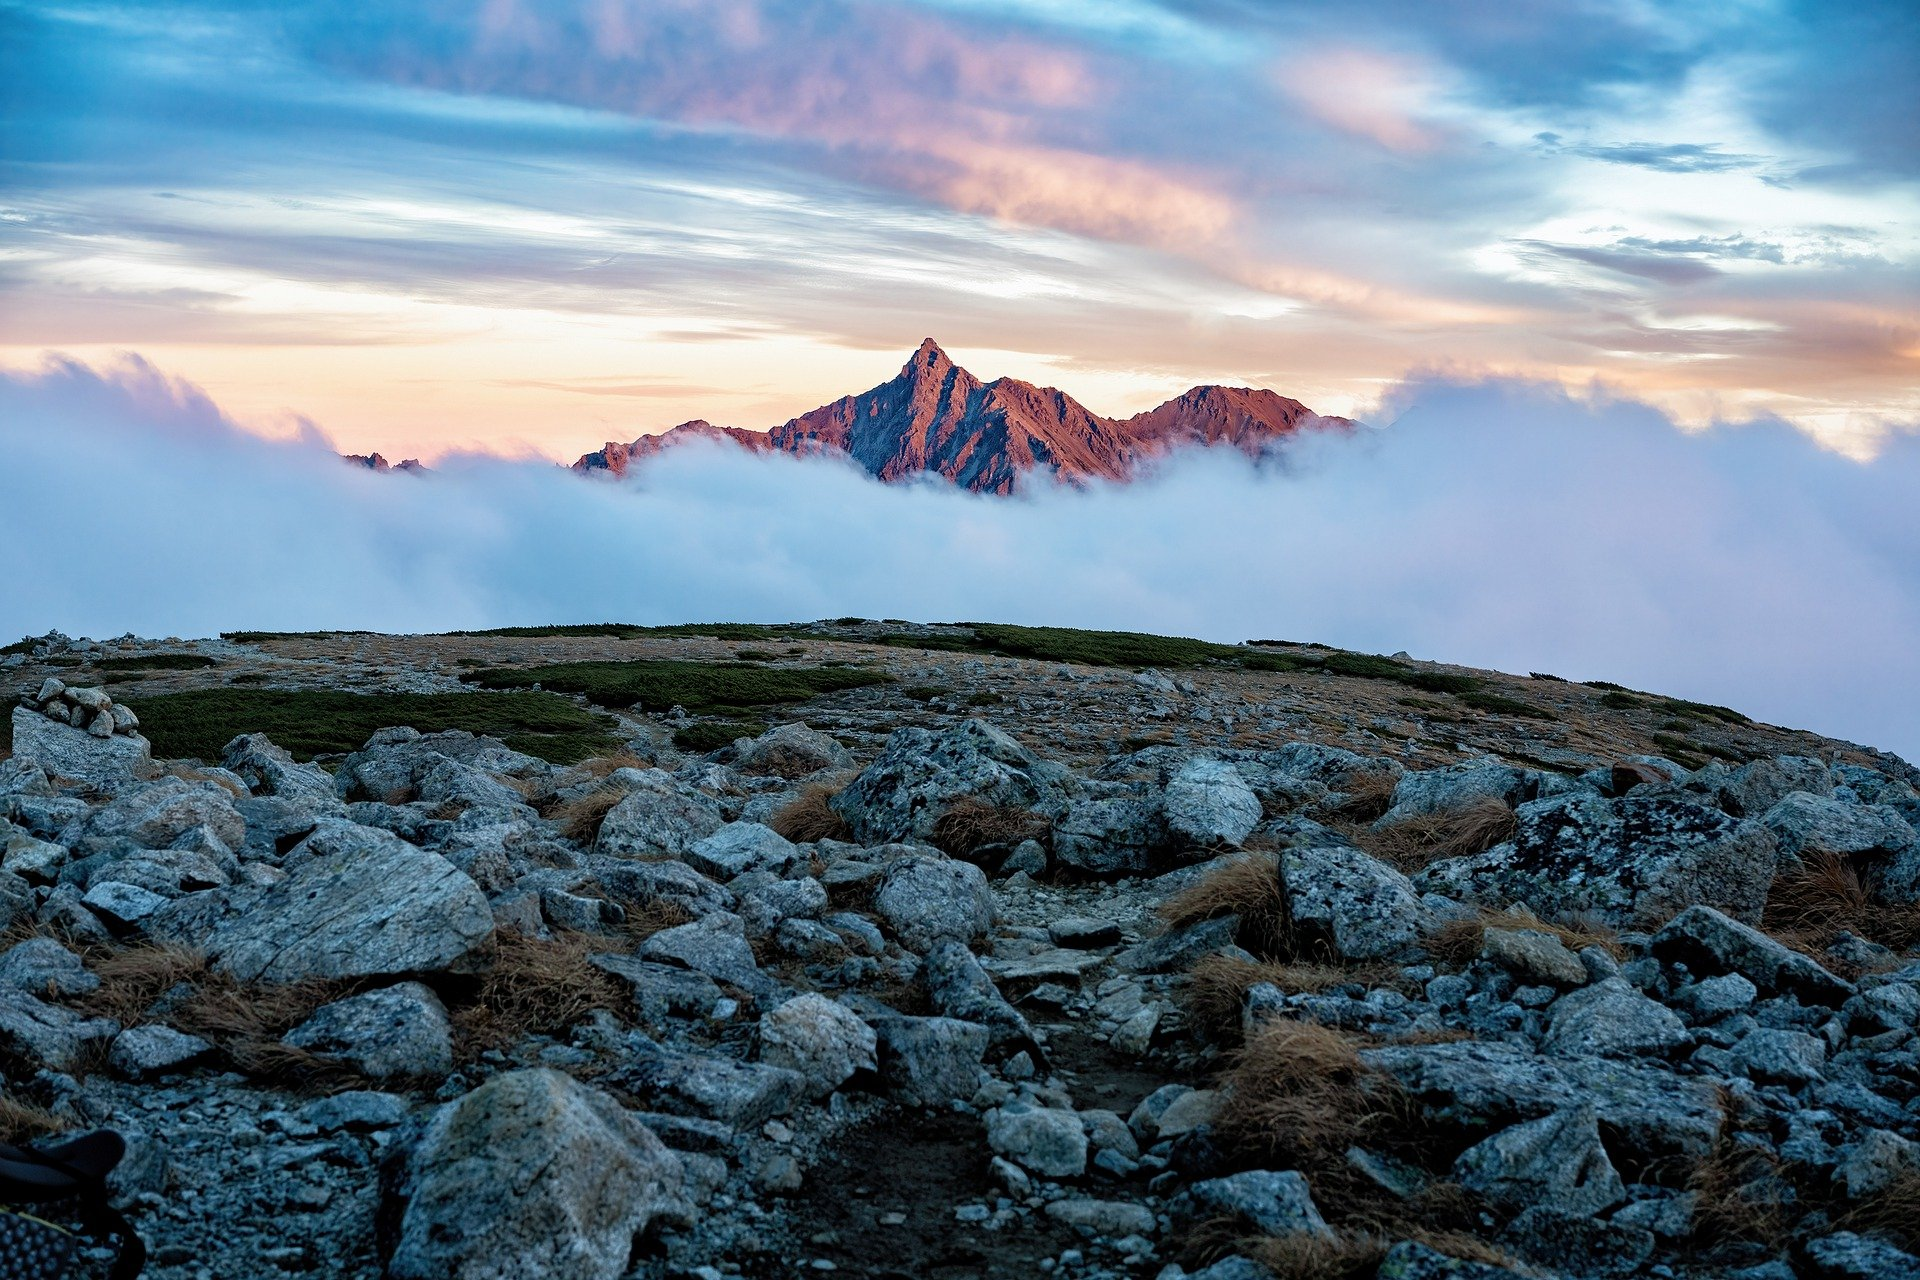
\includegraphics[width=1\linewidth]{landscape}
	\end{minipage}
	\caption{Image caption \cite[S.~5]{buch}}
	\label{img:example_img}
\end{figure}

\subsection{Enumerate}

Enumerate for counted points
\begin{enumerate}
	\item Item 1
	\item Item 2
\end{enumerate}

Use Itemize for bullet points (here also with Header).
\begin{itemize}
	\item \textbf{Header} \\
	Text
	
	\item \textbf{Header} \\
	Text
\end{itemize}

\section{Tables}


\vspace{1em}
\begin{table}[H]
	\centering
	\begin{tabular}{l|cccc}
		\toprule
		\multicolumn{1}{c}{\textbf{Netz}} 
		& \multicolumn{1}{c}{\textbf{Number}}
		& \multicolumn{1}{c}{\textbf{Ratio}}
		& \multicolumn{1}{c}{\textbf{RatioB}} \\
		\midrule
		\multirow{4}{*}{Alpha}
		& 240 & 0\% & 100\% \\
		& 241 & 0\% & 100\% \\
		& 242 & 0\% & 100\% \\
		& 243 & 0\% & 100\% \\
		\cmidrule(lr){1-1}
		\cmidrule(lr){2-4}
		\multirow{4}{*}{Beta}
		& 245 & 1,5\% & 0\% \\
		& 246 & 2,5\% & 0\% \\
		& 247 & 95,5\% & 0\% \\
		& 248 & 0,5\% & 0\% \\
		\bottomrule
	\end{tabular} 
	\captionof{table}[Caption for List of Tables]
    {Caption beneath the table.}
	\label{tab:example_table}
\end{table}


\vspace{1em}
\begin{table}[H]
	\centering
	\begin{tabular}{l|cccc}
		\toprule
		\multicolumn{1}{c}{\textbf{Number}} 
		& \multicolumn{1}{c}{\textbf{Ratio}}
		& \multicolumn{1}{c}{\textbf{RatioB}} 
		& \multicolumn{1}{c}{\textbf{RatioC}}
		& \multicolumn{1}{c}{\textbf{RatioD}}\\
		\midrule
		240 	& 0\% & 100\% & 48\% & 0\% \\
		247 	& 0\% & 100\% & 51\% & 0\% \\
		\bottomrule
	\end{tabular} 
	\captionof{table}[Second Example]
    {Second Table for Examples.}
	\label{tab:vergleich_netz_alpha_vs_beta}
\end{table}

\end{document}

\appendix

\backmatter


\end{document}

